\documentclass[10pt,a4paper]{beamer}

\usepackage[utf8]{inputenc}
\usepackage[russian]{babel}
\usepackage[OT1]{fontenc}
\usepackage{amsmath}
\usepackage{amsfonts}
\usepackage{amssymb}
\usepackage{makeidx}
\usepackage{graphicx}
\usepackage{xcolor}
\usepackage{multirow}
\usepackage{framed}

\definecolor{shadecolor}{cmyk}{0,0,0,1}

\titlegraphic{
   
\includegraphics[width=4cm]{images/sfera.jpg}
}

\author{Николай Анохин \and Михаил Фирулик}
\title{Введение в Data Science \\ Занятие 4. Naive Bayes \\ и классификация текстов}

\beamertemplatenavigationsymbolsempty

\begin{document}

\maketitle

\logo{
    
\includegraphics[width=4cm,keepaspectratio]{images/sfera.jpg}\hspace{0.45em}
}

% ============================================== %

\begin{frame}{План занятия}

\tableofcontents

\end{frame}

% ============================================== %

\section{Обработка текстов}

% ============================================== %

\begin{frame}{Data Mining vs Text Mining}

	\begin{columns}[T]
    \begin{column}{.5\textwidth}
   	Data Mining: \\ извлечение {\it неочевидной} информации

	\vspace{1em}
	Text Mining: \\ извлечение {\it очевидной} информации

\vspace{1em}
Трудности
\begin{itemize}
\item Огромные объемы
\item Отстутсвие структуры
\end{itemize}
	    
    \end{column}
    \begin{column}{.5\textwidth}
    \vspace{1em}
    
\includegraphics[scale=0.06]{images/books.jpg}    
    \end{column}
  \end{columns}

\end{frame}

% ============================================== %

\begin{frame}{Задачи Text Mining}

\begin{itemize}
\item Суммаризация текста \\
{\it аггрегация новостей}
\item Классификация и кластеризация документов \\
{\it категоризация, фильтрация спама, эмоции}
\item Извлечение метаданных \\
{\it определение языка, автора, тегирование}
\item Выделение сущностей \\
{\it места, люди, компании, почтовые адреса}
\end{itemize}

\end{frame}

% ============================================== %

\begin{frame}{Этапы обработки текста}

\begin{center}
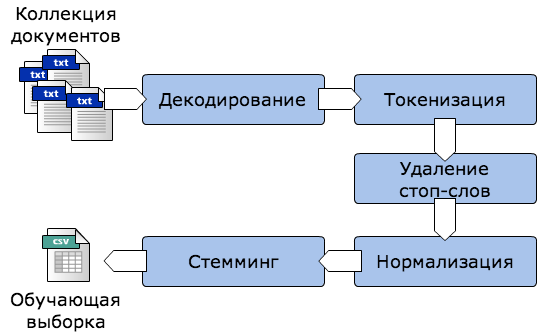
\includegraphics[scale=0.5]{images/textm.png}
\end{center}

\end{frame}

% ============================================== %

\begin{frame}{Декодирование}

\begin{block}{Def.}
перевод последовательности байт в последовательность символов
\end{block}

\begin{itemize}
\item Распаковка \\
{\it plain/.zip/.gz/...}
\item Кодировка \\
{\it ASCII/utf-8/Windows-1251/...}
\item Формат \\
{\it csv/xml/json/doc...}
\end{itemize}

Кроме того: что такое документ?

\end{frame}

% ============================================== %

\begin{frame}{Разбиение на токены}

\begin{block}{Def.}
разбиение последовательности символов на части (токены), возможно, исключая из рассмотрения некоторые символы
\end{block}

\vspace{1em}
{\it Наивный подход:} разделить строку пробелами и выкинуть знаки препинания
\begin{quote}
Трисия любила {\bf Нью-Йорк}, поскольку любовь к Нью-Йорку могла положительно повлиять на ее карьеру.
\end{quote}

{\it Проблемы:}
\begin{itemize}
\item n.anokhin@corp.mail.ru, 127.0.0.1
\item С++, C\#
\item {\it York University} vs {\it New York University}
\item Зависимость от языка (``Lebensversicherungsgesellschaftsangestellter'', ``l'amour'')
\end{itemize}

{\it Альтернатива:} n-граммы

\end{frame}

% ============================================== %

\begin{frame}[fragile]{Разбиение на токены}

\begin{shaded}
{\color{green}
\begin{verbatim}
>>> from nltk.tokenize import RegexpTokenizer
>>> tokenizer = RegexpTokenizer('\w+|[^\w\s]+')
>>> s = u'Трисия любила Нью-Йорк, поскольку любовь \
... к Нью-Йорку могла положительно повлиять на ее карьеру.'
>>> for t in tokenizer.tokenize(s)[:7]: print t + " ::",
... 
Трисия :: любила :: Нью :: - :: Йорк :: , :: поскольку ::
\end{verbatim}
}
\end{shaded}

\end{frame}

% ============================================== %

\begin{frame}[fragile]{Стоп-слова}

\begin{block}{Def.}
Наиболее частые слова в языке, не содержащие никакой информации о содержании текста
\end{block}

\begin{shaded}
{\color{green}
\begin{verbatim}
>>> from nltk.corpus import stopwords
>>> for sw in stopwords.words('russian')[1:20]: print sw,
... 
в во не что он на я с со как а то все она так его но да ты
\end{verbatim}
}
\end{shaded}

\vspace{1em}
Проблема: ``To be or not to be"

\end{frame}

% ============================================== %

\begin{frame}[fragile]{Нормализация}

\begin{block}{Def.}
Приведение токенов к единому виду для того, чтобы избавиться от поверхностной разницы в написании
\end{block}

\vspace{1em}
Подходы
\begin{itemize}
\item сформулировать набор правил, по которым преобразуется токен
\begin{quote}
Нью-Йорк $\rightarrow$ нью-йорк $\rightarrow$ ньюйорк $\rightarrow$ ньюиорк
\end{quote}
\item явно хранить связи между токенами
\begin{quote}
машина $\rightarrow$ автомобиль, Windows $\not \rightarrow$ window
\end{quote}
\end{itemize}

\end{frame}

% ============================================== %

\begin{frame}[fragile]{Нормализация}

\begin{shaded}
{\color{green}
\begin{verbatim}
>>> s = u'Нью-Йорк'
>>> s1 = s.lower()
>>> print s1
нью-йорк
>>> s2 = re.sub(ur"\W", "", s1, flags=re.U)
>>> print s2
ньюйорк
>>> s3 = re.sub(ur"й", u"и", s2, flags=re.U)
>>> print s3
ньюиорк
\end{verbatim}}
\end{shaded}

\end{frame}

% ============================================== %

\begin{frame}{Стемминг и Лемматизация}

\begin{block}{Def.}
Приведение грамматических форм слова и однокоренных слов к единой основе (lemma): 
\begin{itemize}
\item Stemming -- с помощью простых эвристических правил
\begin{itemize}
\item Porter (1980) \\
5 этапов, на каждом применяется набор правил, таких как
\[
sses \rightarrow ss \quad (\text{caresses}\rightarrow\text{caress})
\]
\[
ies \rightarrow i \quad (\text{ponies}\rightarrow\text{poni})
\]
\item Lovins (1968)
\item Paice (1990)
\item еще 100500
\end{itemize}
\item Lemmatization -- с использованием словарей и морфологического анализа
\end{itemize}
\end{block}

\end{frame}

% ============================================== %

\begin{frame}[fragile]{Стемминг}

\begin{shaded}
{\color{green}
\begin{verbatim}
>>> from nltk.stem.snowball import PorterStemmer
>>> s = PorterStemmer()
>>> print s.stem('tokenization'); print s.stem('stemming')
token
stem
>>> from nltk.stem.snowball import RussianStemmer
>>> r = RussianStemmer()
>>> print r.stem(u'Авиация'); print r.stem(u'национальный')
авиац
национальн
\end{verbatim}}
\end{shaded}

\begin{block}{Наблюдение}
для сложных языков лучше подходит лемматизация
\end{block}

\end{frame}

% ============================================== %

\begin{frame}{Heap's law}

\[
M = k T^\beta, \;M \text{ -- размер словаря}, \; T \text{ -- количество слов в корпусе}
\]
\[
30 \leq k \leq 100, \; b \approx 0.5
\]


\begin{center}
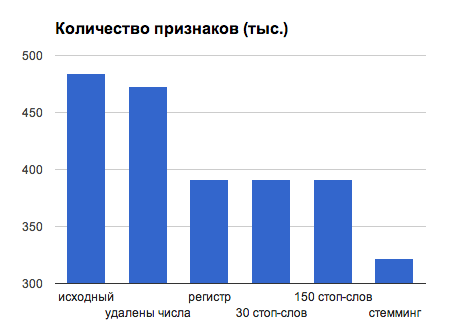
\includegraphics[scale=0.35]{images/dim.png}\;
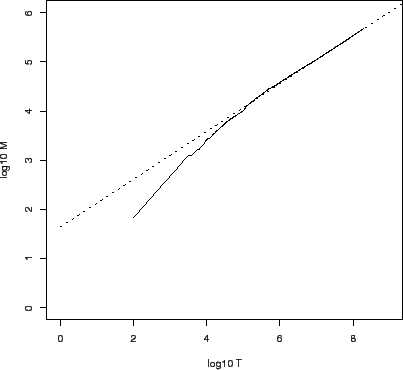
\includegraphics[scale=0.3]{images/heaps.png}
\end{center}

\end{frame}

% ============================================== %

\begin{frame}{Представление документов}

{\bf Boolean Model.} Присутствие или отсутствие слова в документе

\vspace{1em}
{\bf Bag of Words.} Порядок токенов не важен
\begin{quote}
Погода была ужасная, принцесса была прекрасная. \\ Или все было наоборот?
\end{quote}

Координаты
\begin{itemize}
\item Мультиномиальные: количество токенов в документе
\item Числовые: взвешенное количество токенов в документе
\end{itemize}

\end{frame}

% ============================================== %

\begin{frame}{Zipf's law}

\begin{columns}[T]
    \begin{column}{.5\textwidth}
   	$t_1, \ldots, t_N$ -- токены, отранжированные по убыванию частоты
   	
	$f_1, \dots, f_N$ -- соответствующие частоты

	\vspace{1em}
	\begin{framed}
	{\bf Закон Ципфа}
	\[
	f_i = \frac{c}{i^k}
	\]	
	\end{framed}
	
	Что еще? Посещаемость сайтов, количество друзей, население городов...
	    
    \end{column}
    \begin{column}{.5\textwidth}
    \vspace{1em}
    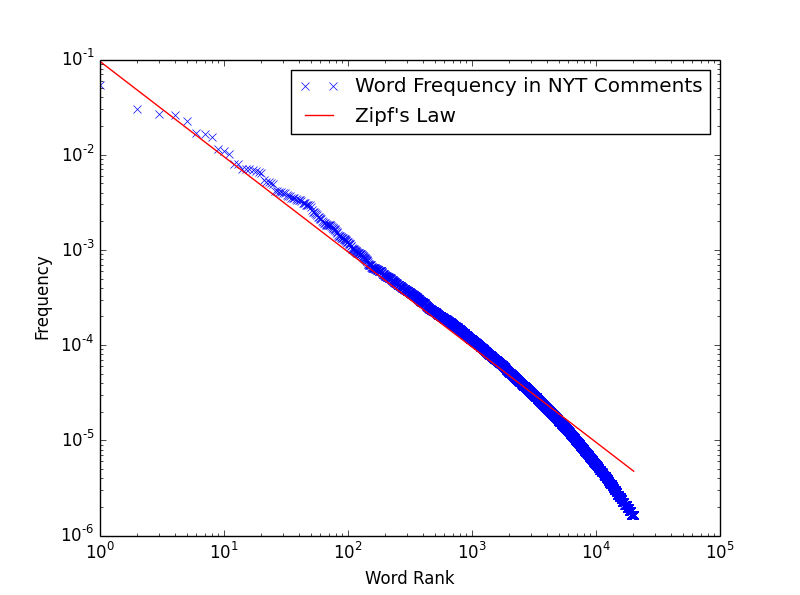
\includegraphics[scale=0.3]{images/zipf.png}    
    \end{column}
  \end{columns}

\end{frame}

% ============================================== %

\begin{frame}{Задача}

Дана коллекция, содержащая $10^6$ (не уникальных) токенов. Предполагая, что частоты слов распределены по закону
\[
f_i = \frac{c}{(i + 10)^2},
\]
оцените
\begin{itemize}
\item количество вхождений наиболее часто встречающегося слова
\item количество слов, котоые встречаются минимум дважды
\end{itemize}

\vspace{1em}
{\it Подсказка: $\sum_{i=11}^{\infty}\frac{1}{i^2} \approx 0.095$}

\end{frame}

% ============================================== %

\begin{frame}{BoW \& TF-IDF}

\vspace{1em}
Количество вхождений слова $t$ в документе $d$
\[
TF_{t,d} = term\!\!-\!\!frequency(t, d)
\]
Количество документов из $N$ возможных, где встречается $t$
\[
DF_t = document\!\!-\!\!fequency(t)
\]
\[
IDF_t = inverse\!\!-\!\!document\!\!-\!\!frequency(t) = \log \frac{N}{DF_t}
\]
TF-IDF
\[
TF\!\!-\!\!IDF_{t,d} = TF_{t,d} \times IDF_t
\]
\begin{exampleblock}{Пример}
Коллекция документов: $\text{Cersei Lannister}$, $\text{Tyrion Lannister}$ \\
$d_1 = \{\text{cersei:}1,\text{tyrion:}0,\text{lannister:}0\}$ \\
$d_2 = \{\text{cersei:}0,\text{tyrion:}1,\text{lannister:}0\}$
\end{exampleblock}

\end{frame}

% ============================================== %

\section{Naive Bayes}

% ============================================== %

\begin{frame}{Байесовский классификатор}

Дано

$\mathbf{x} \in \mathbf{X}$ -- описание документа $d$ из коллекции $D$ \\
$C_k \in C, \; k = 1,\ldots,K$ -- целевая переменная

\vspace{1em}
Теорема Байеса
\[
P(C_k | \textbf{x}) = \frac{p(\textbf{x} | C_k) p(C_k)}{p(\textbf x)} \propto p(\textbf{x} | C_k) p(C_k)
\]
Принцип Maximum A-Posteriori
\[
C_{MAP} = \arg \max_k p(C_k | \textbf{x})
\]

\end{frame}

% ============================================== %

\begin{frame}{Naive Bayes}

$X_j$ -- токен на $j$-м месте в документе $\mathbf{x}$,
$x_i \in V$ -- слово из словаря $V$

\vspace{1em}
Предположения
\begin{enumerate}
\item conditional independence 
\[
p(X_i=x_i, X_j=x_j | C_k) = p(X_i=x_i | C_k) p(X_i=x_i | C_k)
\]
\item positional independence
\[
P(X_i=x_i | C_k) = P(X_j=x_i | C_k) = P(X = x_i | C_k)
\]
\end{enumerate}

Получаем
\[
p(\mathbf{x} | C_k) = p(X_1=x_1, \ldots, X_{|\mathbf{x}|}=x_{|\mathbf{x}|} | C_k) = \prod_{i=1}^{|\mathbf{x}|} p(X = x_i | C_k)
\]

\begin{block}{Почему NB хорошо работает?}
Корректная оценка дает правильное предсказание, но правильное предсказание {\it не требует} корректной оценки
\end{block}

\end{frame}

% ============================================== %

\begin{frame}{Варианты NB}

MAP
\[
C_{MAP} = \arg \max_k \prod_{i=1}^{|\mathbf{x}|} p(X = x_i | C_k) P(C_k) = 
\]
\[
= \arg \max_k \left[ \log P(C_k) + \sum_{i=1}^{|\mathbf{x}|} \log P(X = x_i | C_k) \right]
\]
Априорные вероятности
\[
P(C_k) = N_{C_k}/{N}
\]
Likelihood $p(X = x_i | C_k)$
\begin{itemize}
\item BernoulliNB $P(X = x_i | C_k) = D_{x_i, C_k} / D_{C_k}$, $D$ -- кол-во документов
\item MultinomialNB $P(X = x_i | C_k) = T_{x_i, C_k} / T_{C_k}$, $T$ -- кол-во токенов
\item GaussianNB $P(X = x_i | C_k) = \mathcal{N}(\mu_k, \sigma_k^2)$, параметры из MLE
\end{itemize}

\end{frame}

% ============================================== %

\begin{frame}{Обучение NB}

\texttt{train\_nb($D$, $C$):}

\texttt{\quad $V = $ словарь токенов из $D$}

\texttt{\quad $N = $ количество документов в $D$}

\texttt{\quad for $C_k \in C$:}

\texttt{\quad\quad $N_{C_k} = $ количество документов класса $C_k$}

\texttt{\quad\quad $p(C_k) = N_{C_k}/N$}

\texttt{\quad\quad $D_{C_k} = $ документы класса $C_k$}

\texttt{\quad\quad for $x_i \in V$:}

\texttt{\quad\quad\quad $p(X = x_i | C_k) = $ считаем согласно выбранному варианту}

\texttt{\quad возвращаем $V$, $p(C_k)$, $p(X=x_i | C_k)$}

\vspace{1em}
Алгоритмическая сложность: $O(|D| \langle |\mathbf{x}| \rangle + |C||V|)$

\end{frame}

% ============================================== %

\begin{frame}{Применение MultinomialNB}

\texttt{apply\_nb($d$, $V$, $p(C_k)$, $p(x_i | C_k)$, $C$):}

\texttt{\quad $\mathbf{x} = $ разбиваем $d$ на токены, используя $V$}

\texttt{\quad for $C_k \in C$:}

\texttt{\quad\quad $score(C_k | \mathbf{x}) \, +\!\!= \log p(C_k)$}

\texttt{\quad\quad for $x_i \in \mathbf{x}$:}

\texttt{\quad\quad\quad $score(C_k|\mathbf{x})\,+\!\!= \log p(x_i | C_k)$ считаем согласно выбранному варианту}

\texttt{\quad возвращаем $\arg \max score(C_k | \mathbf{x})$}

\vspace{1em}
Алгоритмическая сложность: $O(|C||\mathbf{x}|)$

\end{frame}

% ============================================== %

\begin{frame}{Задача}

\begin{tabular}{l p{7cm} r}
d & Текст & Класс \\
\hline
1 & котики такие котики & мимими \\
2 & котики котики няшки & мимими \\
3 & пушистые котики  & мимими \\
4 & морские котики мокрые & не мимими \\
\hline
5 & котики котики мокрые морские котики & ???
\end{tabular}

\vspace{1em}
С помощью алгоритма MultinomialNB вычислить $p(\text{мимими} | d_5)$

\end{frame}

% ============================================== %

\begin{frame}{Сглаживание}

{\bf Проблема:} $p(\text{пушистые}|\text{не мимими}) = 0$

\vspace{1em}
{\bf Решение:}
\[
p(X = x_i | C_k) = \frac{T_{x_i, C_k} + \alpha}{T_{C_k} + \alpha |V|}
\]
если $\alpha \geq 1$ -- сглаживание Лапласа, если $0 \leq \alpha \leq 1$ -- Лидстоуна

\vspace{1em}
\begin{exampleblock}{Упражнение}
С учетом сглаживания вычислить 
\[
p(\text{пушистые}|\text{не мимими}), \; p(\text{пушистые}|\text{мимими}).
\]
\end{exampleblock}

\end{frame}

% ============================================== %

\begin{frame}{Байесовские сети}

\begin{center}
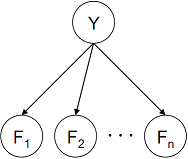
\includegraphics[scale=0.5]{images/naive.png}\quad
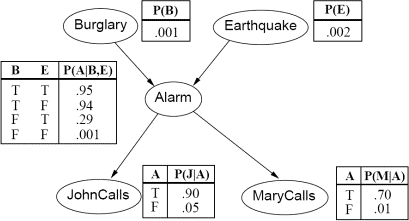
\includegraphics[scale=0.4]{images/network.png}

\vspace{1em}
Naive Bayes \hspace{10em} Bayes Network
\end{center}

\end{frame}

% ============================================== %

\begin{frame}{Итоги}

\begin{itemize}
\item[+] Генеративная модель
\item[+] (Удивительно) неплохо работает
\item[+] Стабилен при смещении выборки (aka concept drift)
\item[+] Оптимальный по производительности
\end{itemize}

\begin{itemize}
\item[--] Наивные предположения
\item[--] Требует отбора признаков
\end{itemize}

\end{frame}

% ============================================== %

\begin{frame}{Определение языка текста}

Определение языка на основании $n$-грамм

\begin{itemize}
\item Нормализация \\
{\it Нижний регистр, заменяем акценты на обычные буквы}
\item Токенизация \\
{\it Разбиваем документы на $n$-граммы}
\item Выбор признаков \\
{\it Берем топ-$k$ признаков из каждого языка}
\item Инициализация модели \\
{\it Используем один из вариантов NB из sklearn}
\item Анализ \\
{\it Как зависит точность предсказания от $n$ и $k$?}
\end{itemize}

\end{frame}

% ============================================== %

\begin{frame}{Домашнее задание 3}

\begin{block}{Байесовский классификатор}
Реализовать
\begin{itemize}
\item алгоритм Naive Bayes для задачи классификации
\item алгоритм Naive Bayes для задачи регрессии
\end{itemize}
\end{block}

Варианты: multinomial, bernoulli, gaussian

\vspace{1em}
Ключевые даты
\begin{itemize}
\item До 2014/03/29 00.00 выбрать задачу и ответственного в группе
\item До 2014/04/05 00.00 предоставить решение задания
\end{itemize}

\end{frame}

% ============================================== %

\begin{frame}{Спасибо!}

\begin{center}
{\Large Обратная связь}
\end{center}

\end{frame}

\end{document}